%-----------------------------Base----------------------------%
\documentclass[a4paper]{article}
\usepackage[utf8]{inputenc}
\usepackage[T1]{fontenc}
\usepackage[english]{babel}
\usepackage[autostyle=true]{csquotes} % Required to generate language-dependent quotes in the bibliography
\usepackage{geometry}
\geometry{
	paper=a4paper, % Change to letterpaper for US letter
	inner=2.5cm, % Inner margin
	outer=2.5cm, % Outer margin
	top=2.5cm, % Top margin
	bottom=2.5cm, % Bottom margin
	%showframe,% show how the type block is set on the page
}
\usepackage{booktabs}
%-----------------------------MATH----------------------------%
\usepackage{amsmath}
\usepackage{amssymb}
%-----------------------------FONT----------------------------%
\usepackage{charter}

%-------------------GRAPHIC ---------------------%
\usepackage{float}
\usepackage{graphicx}
\graphicspath{{figures/}}
\usepackage{tikz}
\usepackage{pgfplots}
\pgfplotsset{compat=1.5}

%-------------------THESIS INFORMATION-----------------%

\title{Fluctuations in a Dual Labor Market}
\author{Normann Rion}
\date{\today}

\begin{document}

\maketitle

\begin{abstract}
I build a New-Keynesian DSGE model with a dual labor market. Firms and workers meet through a matching technology à-la Diamond-Mortensen-Pissarides and endogenously choose between an open-ended contract stipulating a firing tax and a less productive and shorter fixed-term contract. As a result, a trade-off between productivity and flexibility arises at the hiring stage. I use classic Bayesian procedures with data from the Euro Area to estimate the model. The latter replicates well the counter-cyclicality of the share of temporary contracts in job creation, as well as more classic features of a dual labor market. The agents react to shocks essentially through the job creation margin and the contractual composition of the hired workers. Moreover, a general-equilibrium effect arises ; the substitution between temporary and permanent contracts at the hiring stage influences the job seekers' stock, which in turn impacts the job creation margins. Inflation dynamics depend on newly hired workers' productivity and contractual composition. Reforms in employment protection legislation entail persistent movements in inflation.
\end{abstract}

\begin{center}
\textsc{PRELIMINARY VERSION : PLEASE DO NOT CIRCULATE}
\end{center}


\section{Introduction}

In the past decades, temporary employment have grown in importance on European labor markets. In France, for example, temporary contracts represented 5 \% of employed workers in the 80s, while it has been fluctuating around 15\% today. Around 80 \% of job creation occurs through temporary contracts nowadays, most of them with a stipulated duration of less than one month\footnote{See Fontaine and Malherbet (2016) \cite{fontaine2016cdd} for an overview of the situation in European countries}. The introduction of temporary contracts along with the existence of employment protection legislation has given birth to labor market dualism ; highly protected open-ended contracts and short fixed-term contracts coexist. This paper studies the implications of this phenomenon on the cycles. To fulfill this ambition, I estimate a New-Keynesian DSGE model with a dual labor market on data concerning the Euro Area.

The contribution is threefold. First of all, from a theoretical point of view, the choice between temporary and permanent contracts is endogenous at the hiring stage. The model is able to account for the contractual composition of hires and its fluctuations. The strong counter-cylicality of the share of temporary contracts in job creation is well-rendered, along more classic labor market moments. Secondly, two main economic mechanisms arise as shocks hit the economy. The possibility to substitute temporary contracts and permanent contracts at the hiring stage plays an important role on impact. This initial substitution effect on the composition of job creation impacts the number of job seekers', which in turn influences the thickness of job creation flows. There is a direct link between fluctuations in composition of job creation and fluctuations in the quantity of job creation. Finally, the newly hired workers' contractual composition and productivity intervene in inflation dynamics. Marginal and transitory reforms on employment protection legislation, which are frequent in the Euro Area, generate persistent and significant movements in inflation. Moreoever, I find that the dual model presents a higher likelihood with respect to its estimated classic counterpart.

The literature is scarce when it comes to consider both a truly endogenous choice between open-ended and fixed-term contracts and fluctuations in a dual labor market. The main references when it comes to study cycles with a dual labor market are the pioneering papers of Sala and Silva (2009) \cite{sala2009flexibility}, Costain, Jimeno and Thomas (2010) \cite{costain2010employment} and Sala, Silvia and Toledo (2012) \cite{SJOE:SJOE1715}. These models either assume that job creation only occurs through temporary contracts, or the share of temporary contracts is constant and exogenously set. 
However, Shimer (2005) \cite{shimer2005cyclical} demonstrated the importance of job creation flows in the understanding of unemployment fluctuations. Moreover, given the overwhelming prominence of temporary contracts in job creation flows, the contractual composition of hires needs to be considered from a policy perspective.

Beyond the study of fluctuations, the literature is rich in approaches to endogeneize the choice between temporary contracts and permanent contracts. Cahuc et al. (2016) \cite{IERE:IERE12167} introduce differences in the life span of workloads across vacancies. Jobs with a short expected duration of profitability are exploited through temporary contracts, whereas jobs with long-lasting prospects of profitability are filled by permanent contracts. Berton and Garibaldi (2012) \cite{berton2012workers} explore the role of labour market ranking in a dual framework. A compromise between flexibility and the vacancy-filling speed leads to the coexistence of temporary and permanent contracts at the equilibrium. Cao et al. (2010) \cite{cao2010fixed} show that highly productive workers are offered permanent contracts, because temporary workers have an incentive to search on the job, which depletes their productivity. Caggese and Cunat (2008), as for them, introduce temporary contracts, which are less productive than permanent contracts by assumption, in firms with a decreasing-return-to-scale technology. As a result, firms hire permanent contracts until the productivity gains are offset by the expected losses from costly separations, and hire temporary contracts beyond that point. My model lies on this productivity-flexibility trade-off in the manner of Rion (2019) \cite{rion2019} ; temporary and permanent contracts coexist on the same labour market, but temporary contracts are less productive than permanent contracts. Permanent contracts are more productive but may become expensive in case of endogenous separation, whereas temporary contracts are less productive while enabling a quicker and cost-less split when a recession strikes. The contract is endogenously chosen between both contracts at the hiring stage depending on an idiosyncratic shock the worker-firm pair draws. Otherwise, the labor market is similar to the classic stand of Mortensen and Pissarides (1994) \cite{mortensen1994job}.

The assumption of an existing contractual productivity wedge is fundamental and deserves justification. The young are over-represented in temporary employment and benefit from a lower tenure. Moreover, temporary contracts present a low probability to be transformed in permanent contracts. Temporary workers are likely to undergo successions of short employment periods and long unemployment spans. Meanwhile, Pissarides (1992) \cite{pissarides1992loss} shows that unemployment periods reduce concerned  workers' skills. This has a negative effect on the productivity of temporary employment. A report from the OECD (2014) \cite{oecd2014} also documented that temporary workers suffer from a depressed access to formation compared with permanent employees. This evidence support our core assumption. 

The study of nominal rigidities along with fluctuations in labor markets constitutes a leafy literature\footnote{See, among many others, Gertler et al. (2008) \cite{gertler2008estimated}, Trigari (2009) \cite{trigari2009equilibrium}, Blanchard and Gali (2010) \cite{blanchard2010labor} and Christiano et al. (2016) \cite{christiano2016unemployment} among others}, where dualism has never been considered, as far as I know.  For the sake of comparability, I stick to Zanetti and Thomas (2009) \cite{THOMAS2009885} when it comes to the New-Keynesian block. They introduce employment protection legislation in a Mortensen-Pissarides model along with nominal rigidities. I depart from their analyses by considering transition instead of steady-state decomposition of volatilities, and find that inflation movements can be substantial and persistent in response to reforms in employment protection legislation in opposition to what their conclusions suggest.

The paper is organized as follows. Section 2 presents the model. Secton 3 exposes the calibration and estimation procedure. Section 4 displays the main results of our analysis. Section 5 concludes.  

\section{Model}

The model follows a discrete timing and embeds 4 types of agents ; the households, the firms, the government and the fiscal authority. Three types of firms coexist. Perfectly competitive final good producers generate the homogenous good valued by households for consumption and investment. This final good producers aggregate the differentiated goods produced by the retailers. The latter retailers are monopolistically competitive and transform the homegeneous intermediate good into a differentiated retail good. Intermediate firms produce the associated intermediate good and experience perfect competition. These intermediate firms, which we will simply call firms in what follows, use labor as their only input. I rely on Mortensen and Pissarides (1994) \cite{mortensen1994job} as for the shaping of the labor market. Workers can be either employed or unemployed and are identical. There is no on-the-job search, which implies that only unemployed workers search for a job. Firms, as for them, can employ workers and post vacancies in order to meet the former. The number of contacts per period is $m(e,v)$, where $e$ is the number of job-seekers and $v$ is the number of vacancies. A classic measure of the matching activity is the labor market tightness $\theta =  v/e$. The matching function $m$ has constant returns to scale, which enables the definition of the vacancy-worker meeting probability $p(\theta)$ on the job seekers' side and its counterpart $q(\theta)$ on the firms' side.

\begin{align*}
q &= \frac{m\left(e,v\right)}{v} = m \left( \theta^{-1}, 1\right)\\
p &= \frac{m\left(e,v\right)}{e} = m \left( 1, \theta\right) = \theta q(\theta)\\
\end{align*}

As usual in this literature, the workers' vacancy-worker meeting probability is increasing, whereas the firms' vacancy-worker meeting probability is decreasing. Note that these meeting probabilities are not the classic job-finding and vacancy-filling probabilities. Indeed, in this paper, a match does not necessarily lead to a productive firm-worker association. When a firm and a worker meet, the idiosyncratic productivity of the match $z$ is revealed. The latter is drawn from a distribution with cdf $G$.

An important aspect of the model is the timing assumption. At the beginning of the period, agents learn the value of shocks. According to these new information, firms manage their workforce ; they may lay off workers and post vacancies. Next, new matches are revealed. Importantly, a paired firm and worker may return to search if the revealed productivity of the match is disappointing. Moreover, workers fired in the current period are able to participate to the present meeting round. This assumption is important to avoid an underestimation of the labor market flows, especially when the length of one periods is long compared  with the average length of a job. Indeed, temporary jobs last 1.5 months on average in France, which might become a problem when the model is estimated on a quarterly basis and the workers must stay unemployed at least one period to be able to find a job again. Then, production is carried out, firms pay for wages and firing costs. At this point, households consume, and so ends the period. Figure \ref{timing} sums up the timing in the economy. 

\begin{figure}[H]
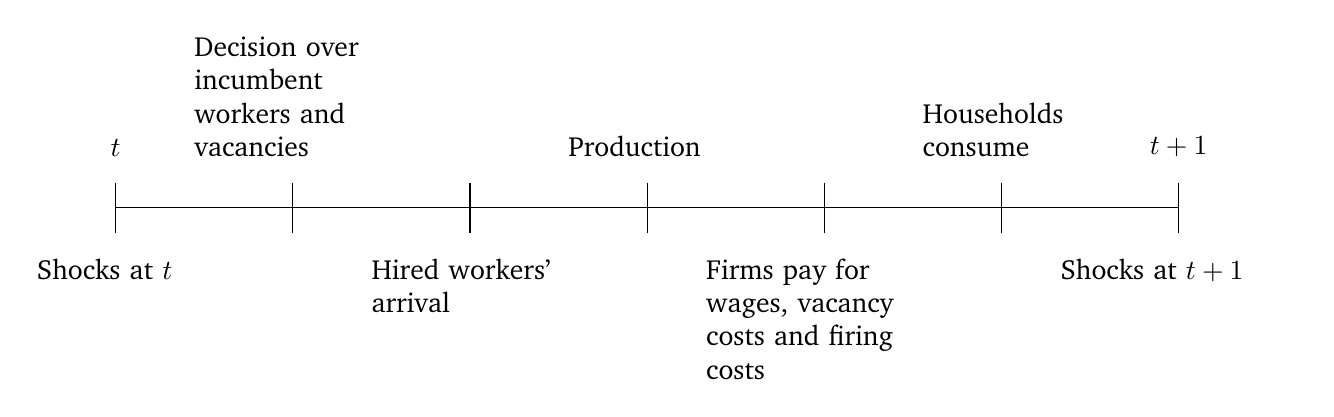
\begin{tikzpicture}[scale = 0.9]
%draw horizontal line
\draw (0cm,0cm) -- (15cm,0cm);
draw vertical lines
\foreach \x in {0, 2.5, 5, 7.5, 10, 12.5, 15}{
   \draw (\x,10pt) -- (\x,-10pt);
}
\draw (0,0) node[below=15pt, text width=2cm] {Shocks at $t$} node[above=15pt] {$t$};
\draw (2.5,0) node[above=15 pt, text width=2.5cm] {Decision over incumbent workers and vacancies};
\draw (5,0) node[below=15pt, text width=2.5cm] {Hired workers' arrival};
\draw (7.5,0) node[above=15pt, text width=2cm] {Production};
\draw (10,0) node[below=15pt, text width=3cm] {Firms pay for wages, vacancy costs and firing costs};
\draw (12.5,0) node[above=15pt, text width=2cm] {Households consume};
\draw (15,0) node[below=15pt, text width=3cm] {Shocks at $t+1$} node[above=15pt] {$t+1$};
\end{tikzpicture}
\label{timing}
\caption{The timing of the economy}
\end{figure}

\subsection{Households}

Households are identical and constitute a continuum represented  by the interval $(0,1)$. Perfect pooling of revenues leads to an equal consumption for all households, as in Merz (1995) and Andolfatto (1996). Households hold the firms, consume the homogeneous good produced by final good firms and save using one-period nominal bonds. They earn wages, unemployment benefits, interests on their savings and pay lump-sum taxes. As a result, the households' program boils down to

\begin{align*}
&\max_{\left\{c_t, B_{t+1} \right\}_{t=0}^{+\infty}} \mathbb{E}_0 \sum_{t = 0}^{+\infty} \beta^t u\left(c_t\right)\\
&\text{s.t } c_t + \frac{B_{t+1}}{P_t} = R_{t-1} \frac{B_{t}}{P_t} + \overline{w_t^p}_t n_t^p + \overline{w_t^f} n_t^f + b u_t + \Pi_t - \tau_t
\end{align*}

$C_t$ marks down consumption.\footnote{I omit the subscript $i$ since all households share the same allocations for consumption and savings.} $B_{t}$ is the amount of nominal bond holdings at the beginning of period $t$, with the associated interest rate $i_t$ between $t-1$ and $t$. $\overline{w_t^p}$, $\overline{w_t^f}$ and $\overline{w_t}$ are respectively the average real wages for permanent jobs, temporary jobs and all workers. $b$ denotes the unemployment benefits. $n_t^p = \int_{0}^{1} n_{i,t}^p di$ is the aggregate permanent employment and $n_t^f$ denotes its temporary counterpart. $u_t$ marks down the measure of unemployed households. Firms transfer their profits to households through $\Pi_t$, while the government taxes $\tau_t$ to finance the payment of unemployment benefits.

The first order conditions with respect to $c_t$ and $B_{t+1}$ lead to the following Euler equation

\begin{align}
&\lambda_t = \beta \mathbb{E}_t \left[ R_{t} \frac{P_t}{P_{t+1}} \lambda_{t+1} \right] \label{euler_eq}\\
&\lambda_t = u' \left( c_t \right)\label{def_up}
\end{align}

The resulting firms' discount factor is $\beta_{t,s} = \beta^{s-t} \lambda_s / \lambda_t$ since households own the firms.

\subsection{Final good firms}

Final good firms are identical and compete to produce the good consumed by the households. They use a Dixit-Stiglitz aggregator as technology to put together retail goods and produce $Y_t$

\begin{equation}
Y_t = \left( \int_{0}^{1} Y_{i,t}^{\frac{\epsilon_t - 1}{\epsilon_t}} di \right)^{\frac{\epsilon_t}{\epsilon_t} - 1} \label{con_fin}
\end{equation}

where $\epsilon_t$ is the elasticity of substitution between retail goods.

The firm takes as given the price of the retail goods $P_{i,t}$ and the price of the final good $P_t$ and maximizes its profits with respect to the components of its input $\left\{Y_{i,t}\right\}_{i\in(0,1)}$ under the constraint \eqref{con_fin}. Therefore, the program of the final good firm boils down to

\begin{align*}
&\max_{\left\{Y_{i,t}\right\}_{i\in[0,1]}} P_t Y_t - \int_{0}^{1} P_{i,t} Y_{i,t} di\\
&\text{subject to \eqref{con_fin}}
\end{align*}

The subsequent first order condition provides an expression for the demand of the retail good $i$

\begin{equation}
Y_{i,t} = \left( \frac{P_{i,t}}{P_t} \right)^{-\epsilon_t} Y_t \label{ret_dem}
\end{equation}

\subsection{Retailers}

Retailers buy goods from intermediate firms and sell the obtained production to final good producer\footnote{At this step, it is possible to introduce capital so as to extend the model.}. They are monopolistically competitive and lie on the interval $(0,1)$. The only thing they accomplish is the one-to-one transformation of the intermediate good into a retail good. Denoting $X_{i,t}$ the retailer $i$'s input in the intermediate good, the production technology writes

\begin{equation*}
Y_{i,t} = X_{i,t}
\end{equation*}

As a result, retailers face a marginal cost that equals the relative price of the intermediate good $\phi_t$. I assume that these firms face a staggered price adjustment à-la Calvo (1983) \cite{calvo1983staggered}.

\begin{align*}
P_{i,t} = \left\{ \begin{array}{ll}
P_{i,t-1} & \text{ with probability } \psi\\
P_{i,t}^* & \text{ with probability } 1-\psi\\
\end{array}
\right.
\end{align*}

A fraction $\psi$ of retailers is able to adjust its prices to the optimal value $P_{i,t}^*$, whereas the  remaining retailers stick to their former prices. There is no indexation of non-adjusted princes on inflation in this model. Therefore, the price-setting retail firm $i$ at period $t$ experiences the following program

\begin{align*}
&\max_{P_{i,t}^*} \mathbb{E}_{t} \sum_{T = t}^{+\infty} \beta_{t,T} \psi^{T-t} \left( \frac{P_{i,t}^*}{P_T} - \phi_{T} \right) Y_{i,T} \\
&\text{ subject to } Y_{i,T} = \left( \frac{P_{i,t}^*}{P_T} \right)^{-\epsilon_t} Y_T
\end{align*}

where $\beta_{t,s}$ is the retailer's discount factor on time $t$ for a unit of profit earned at time $s$. This leads to the following first order condition

\begin{equation}
\mathbb{E}_{t} \sum_{T = t}^{+\infty} \beta_{t,T} \psi^{T-t} P_T^{\epsilon_T} Y_T \left( \frac{P_{i,t}^*}{P_T} - \mu_T \phi_T \right) = 0 \label{price_eq}
\end{equation}

where $\mu_t = \epsilon_t /(\epsilon_t-1)$ is a mark-up shock such that $log\left( \mu_t \right) = \left(1-\rho_\mu\right) log\left( \epsilon / (\epsilon - 1) \right) + \rho_\mu log \left( \mu_{t-1} \right) + \epsilon_t^{\mu}$, with $\epsilon_t^{\mu} \overset{iid}{\sim} \mathcal{N} \left(0, \sigma_\mu^2 \right)$.

\subsection{Intermediate good firms}

Intermediate good firms are in perfect competition, sell their output to retailers and use labor as input. They can employ one worker or maintain one vacancy. They face an idiosyncratic productivity shock $z_t$, an aggregate productivity shock $A_t$ and use open-end or fixed-term contracts to manage their workforce. $A_t$ follows the process $log\left(A_t\right) = (1-\rho_A) log\left(\overline{A}\right) + \rho_A log\left(A_{t-1}\right) + \epsilon_t^A$, with $\epsilon_t^A \overset{iid}{\sim} \mathcal{N} \left( 0, \sigma_A^2 \right)$.

\paragraph{Open-ended contracts} A continuing open-ended contract delivers the wage $w_{t}^{p}$ and stipulates a firing tax $F_t = \phi_t A_t F$. On each period, an open-ended match may exogenously separate with probability $s$. In this case, the firing cost needs not to be paid. Otherwise, the firm chooses whether it keeps or lays off the worker regarding the idiosyncratic productivity of the match. An endogenous separation entails the payment of the firing cost. If I denote the firm's surplus with a continuing permanent match $J_t^p$ and the present discounted value of a vacancy $V_t$, I get the equation

\begin{align*}
J_t^p \left( z_{t} \right) = \phi_t A_t z_{t} - w_{t}^{p} \left( z_t \right) + \mathbb{E}_{t} \beta_{t,t+1} (1-s) \left\{ \int_{z_{t+1}^p}^{+\infty} J_{t+1}^{p} \left( z \right) dG(z) - G\left(z_{t+1}^p\right) F_{t+1} \right\}
\end{align*}

where $z_t^p$ is the threshold for endogenous separations when it comes to the idiosyncratic productivity of the match. The probability of separation for permanent contracts is thus

\begin{equation}
\xi_t^p = s + (1-s) G\left( z_t^p \right) \label{def_xip}
\end{equation}

In the case of a new match, the expression is the same but the wage is replaced with its entry-level counterpart. The negotiation of the permanent entry-level wage between firms and workers does not imply the payment of a firing cost in case of disagreement, which significantly weakens the threat point of the worker. After one period at the entry-level wage and apart from exogenous separations, the match is converted to a classic continuing permanent match if the idiosyncratic productivity is high enough. Otherwise, the match endogenously separates and the firm pays the firing cost.

\begin{align*}
J_{t}^{0,p} \left( z_{t} \right) = \phi_t A_t z_{t} - w_{t}^{0,p} \left( z_t \right) + \mathbb{E}_{t}  \beta_{t,t+1} (1-s) \left\{ \int_{z_{t+1}^p}^{+\infty} J_{t+1}^{p} \left( z \right) dG(z) - G\left(z_{t+1}^p\right) F_{t+1} \right\}
\end{align*}

\paragraph{Fixed-term contracts} A fixed-term contract stipulates the wage $w_{i,t}^{f}$ and yields a relative productivity with respect to permanent contracts $0 < \rho < 1$. The existence of a productivity gap between temporary and permanent contracts in the data motivates this assumption, as was developed in the introduction.

Similarly to permanent matches, the temporary pair may separate exogenously with a probability $s$, which represents the exogenous probability of returning to unemployment. Otherwise, the match comes to an end with exogenous probability $\delta$, which corresponds to the stipulated termination date of the fixed-term contract. Thus, the transition probability from temporary employment to unemployment is exogenous and can be defined as

\begin{equation*}
\xi^f = s + (1-s)\delta
\end{equation*}

I denote $J_t^f$ the present discounted value of a continuing match under a temporary contract.

\begin{align*}
J_{t}^f \left( z_t \right) = \rho A_t \phi_t z_t - w_{i,t}^{f} \left( z_t \right) + \mathbb{E}_{t} \beta_{t,t+1} \left( 1-\xi^f \right)  \int J_{t+1}^{f} \left( z \right) dG(z)
\end{align*}

\paragraph{Vacancies} In opposition to most of the literature, the choice between a temporary and a permanent contract at the hiring step is explicitly embedded and in endogenous. When paired with a worker, firms can hire through a temporary contract or hire through a permanent contract. They are also able to return searching for a worker and get the chance to be matched with another one on the next period. The following equation bears witness of these possible options.

\begin{equation*}
V_t = - \gamma + q \left( \theta_{t} \right) \int max \left[ J_{t}^{p} \left( z \right) , J_{t}^{f} \left( z \right) ,  E_{t} \beta_{t,t+1} V_{t+1} \right] dG(z)
\end{equation*}

It should be noted that the firing costs only apply if the match is validated in the first place. The potentially ephemeral constitution of a match does not boil down to the payment of firing costs if immediate separation is preferable. Thus, the role of firing costs is not unrealistically exacerbated at the creation stage.  

\subsection{Wage bargaining}

I assume that wages are set each period through a Nash-bargaining process. Thus, denoting $\eta$ the worker's share of the surplus of the match, the sharing rules write

\begin{align*}
&W_t^p \left( z_t \right) = \eta S_t^p \left( z_t \right)\\
&W_t^{0,p} \left( z_t \right) = \eta S_t^{0,p} \left( z_t \right)\\
&W_t^f \left( z_t \right) = \eta S_t^f \left( z_t \right)
\end{align*}

where $W_t^p$ is the worker's surplus from a continuing permanent contract, $W_t^{0,p}$ is the worker's surplus from a new permanent contract and $W_t^{0,p}$ is the temporary worker's surplus. The analogous total surpluses are denoted with $S$ and the proper subscripts and indexes. Total surpluses are defined as the sum of the firm's and the worker's surplus from the match.

\begin{align*}
S_t^p \left( z_t \right) &= J_t^p \left( z_t \right) - \left( V_t - F_t \right) + W_t^p \left( z_t \right) - U_t\\
S_t^{0,p} \left( z_t \right) &= J_t^{0,p} \left( z_t \right) - V_t + W_t^{0,p} \left( z_t \right) - U_t\\
S_t^{f} \left( z_t \right) &= J_t^{f} \left( z_t \right) - V_t + W_t^{f} \left( z_t \right) - U_t\\
\end{align*}

where $U_t$ is the surplus of the unemployed. As intended, the continuing permanent worker's surplus includes the firing cost in case of endogenous separation. This bolsters his threat point in the Nash-bargaining process and pushes up his wage. The new permanent workers does not benefit from this effect since a failure in the bargaining process does not entail the payment of $F_t$.

Using the different definitions of the firms' and the workers' surpluses, the total surpluses write

\begin{align*}
S_t^p \left( z_t \right) = &A_t \phi_t z_t - b + F_t - (1-s) \mathbb{E}_t \beta_{t,t+1} F_{t+1} - \mathbb{E}_t \beta_{t,t+1} \left( 1 - \xi_{t+1}^p \right) \frac{\eta \gamma}{1-\eta}\theta_{t+1}\\
& + (1-s) \mathbb{E}_t \beta_{t,t+1} \int_{z_{t+1}^p}^{+\infty} S_{t+1}^p \left( z' \right) dG\left( z' \right)\\
S_t^{0,p} \left( z_t \right) =& S_t^{p} \left( z_t \right) - F_t\\
S_t^f \left( z_t \right) =& \rho A_t \phi_t z_t - b - \left( 1 - \xi^f \right) \mathbb{E}_t \beta_{t,t+1} \frac{\eta \gamma}{1-\eta}\theta_{t+1} + \left( 1 - \xi^f \right)\mathbb{E}_t \beta_{t,t+1} \int S_{t+1}^f \left( z' \right) dG \left( z' \right)
\end{align*}

Using the expressions for the firms' surpluses along with the expressions for the total surpluses above and the surplus sharing rules, the wages verify

\begin{align*}
w_t^p \left( z_t \right) &= \eta \left( A_t \phi_t z_t + F_t -(1-s)E_t \beta_{t,t+1}F_{t+1} + E_t \beta_{t,t+1} \left( 1-\xi_{t+1}^p \right) \gamma \theta_{t+1} \right) + (1-\eta) b\\
w_t^{0,p} \left( z_t \right) &= \eta \left( A_t \phi_t z_t -(1-s)E_t \beta_{t,t+1} F_{t+1} + E_t \beta_{t,t+1} \left( 1-\xi_{t+1}^p \right) \gamma \theta_{t+1} \right) + (1-\eta) b\\
w_t^f \left( z_t \right) &= \eta \left( \rho A_t \phi_t z_t + \left( 1-\xi^f \right) E_t \beta_{t,t+1} \gamma \theta_{t+1} \right) + (1-\eta) b\\
\end{align*}

The wage of the continuing permanent worker increases with the firing cost. The firing cost acts as a tax on separation but also as an upward force in the continuing permanent worker's threat point in the wage bargaining process. The new permanent worker is penalized with higher firing costs to compensate the future gains of wages in case of continuation. As usual in the Mortensen-Pissarides literature, the labor market tightness increases the outside option of the workers through the enlarged chances of finding a job and the wages raise.

\subsection{Job creation and job destruction}

In this section, I circumscribe the equilibrium characteristics of job creation and job destruction.

I assume that there is free entry on the labor market for firms through the posting of vacancies. At the equilibrium, the asset value of an unfilled vacancy is zero.

\begin{align*}
V_t = 0
\end{align*}

The job creation condition stems from the free-entry condition and the Bellman equation defining the present discounted value of an unfilled vacancy

\begin{align*}
\frac{\gamma}{(1-\eta) q\left( \theta_t \right)} = \int max \left[ S_t^{0,p} \left( z \right) , S_t^{f} \left( z \right), 0\right] dG(z)
\end{align*}

Importantly, the Nash-bargaining rules implies that the whole behaviour of the labor boils down to the total surpluses of matches. The destruction of permanent contracts occurs when the surplus of a continuing match reaches zero. Thus, $z_t^p$ follows

\begin{align*}
S_t^p \left( z_t^p \right) = 0
\end{align*}

Using this definition, the expression for $S_t^p$, as well as an integration by part along with that fact that $\partial S_t^p / \partial z_t = \phi_t$, $z_t^p$ follows

\begin{equation}
A_t \phi_t z_t^p + F_t - (1-s) \mathbb{E}_t \beta_{t,t+1} F_{t+1} + (1-s) \mathbb{E}_t \beta_{t,t+1} A_{t+1} \phi_{t+1} \int_{z_{t+1}^p}^{+\infty} \left[ 1 - G(z) \right] dz = b +\mathbb{E}_t \beta_{t,t+1} \left( 1 - \xi_{t+1}^p \right) \frac{\eta \gamma}{1-\eta}\theta_{t+1} \label{def_zp}
\end{equation}

Moreover, at the hiring stage, the profitability of temporary contracts becomes actual when the productivity shock exceeds $z_t^f$ such that

\begin{align*}
S_t^{f} \left( z_t^f \right) &= 0\\
\end{align*}

Using the same procedure as for $z_t^p$, the definition of $z_t^f$ can rewritten as

\begin{equation}
\rho A_t \phi_t z_t^f + \left( 1 - \xi^f \right) \rho \mathbb{E}_t \beta_{t,t+1} A_{t+1}  \phi_{t+1} \left[ \mathbb{E}_z - z_{t+1}^f \right] = b + \left( 1 - \xi^f \right) \mathbb{E}_t \beta_{t,t+1} \frac{\eta \gamma}{1-\eta}\theta_{t+1} \label{def_zf}
\end{equation} 

Analogously, the profitability of new permanent contracts reaches zero at the threshold $z_t^c$, such that

\begin{equation*}
S_t^{0,p} \left( z_t^c \right) = 0
\end{equation*}

Using the definition of $S_t^{0,p}$ and the fact that $S_t^p \left( z_t^p \right) = 0$, the definition of $z_t^c$ can be rephrased as

\begin{equation}
A_t \phi_t z_t^c = A_t \phi_t z_t^p + F \label{def_zc}
\end{equation}


\begin{figure}[t]
\begin{center}
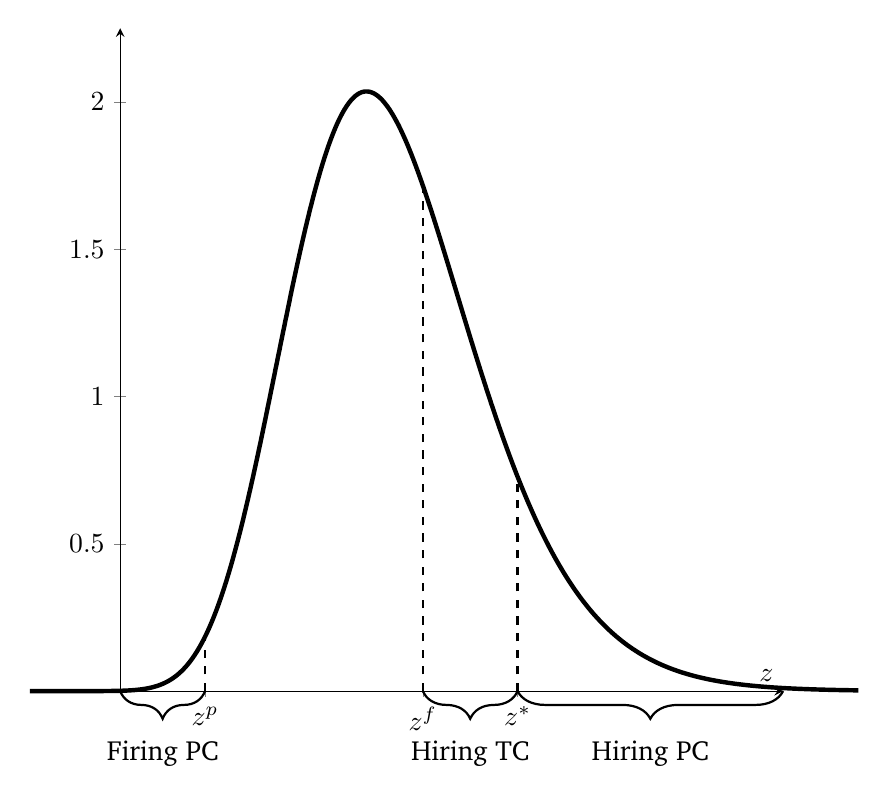
\begin{tikzpicture}

\newcommand\zp{0.62}
\newcommand\zf{1.08}
\newcommand\zs{1.28}
\newcommand\sigz{0.2}

\begin{axis}[
clip=false,
height = 10cm,
width = 10cm,
xlabel = $z$,
ylabel = {},	
xmin = exp(\sigz^2)-3*\sigz,
xmax = exp(\sigz^2)+4*\sigz,
ymin = 0.,
ymax = 2.25,
axis lines = middle,
legend pos= outer north east,
xtick = {\zp,\zf,\zs},
xticklabels={$z^p$,$z^f$,$z^*$}
]

\addplot[color = black,ultra thick,samples=1000,domain = 0.25:2.] { exp(-0.5*ln(x)^2/(0.2^2)) / (x*0.2*sqrt(2*pi))} ;
\addplot [color = black,thick,dashed]  coordinates { (\zp,0.) (\zp,{exp(-0.5*ln(\zp)^2/(0.2^2)) / (\zp*0.2*sqrt(2*pi))} ) };
\addplot [color = black,thick,dashed]  coordinates { (\zf,0.) (\zf,{exp(-0.5*ln(\zf)^2/(0.2^2)) / (\zf*0.2*sqrt(2*pi))} ) };
\addplot [color = black,thick,dashed]  coordinates { (\zs,0.) (\zs,{exp(-0.5*ln(\zs)^2/(0.2^2)) / (\zs*0.2*sqrt(2*pi))} ) };
\draw [thick,decoration={brace,mirror,amplitude = 10pt},decorate] (axis cs:{exp(\sigz^2)-3*\sigz},0.) -- (axis cs:\zp,0.) node[midway,below,yshift=-0.5cm] {Firing PC};
\draw [thick,decoration={brace,mirror,amplitude = 10pt},decorate] (axis cs:\zf,0.) -- (axis cs:\zs,0.) node[midway,below,yshift=-0.5cm] {Hiring TC};
\draw [thick,decoration={brace,mirror,amplitude = 10pt},decorate] (axis cs:\zs,0.) -- (axis cs:{exp(\sigz^2)+4*\sigz},0.) node[midway,below,yshift=-0.5cm] {Hiring PC};
\end{axis}

\end{tikzpicture}
\end{center}
\caption{The PDF of idiosyncratic shocks and the location of thresholds}
\label{pdf}
\end{figure}

The choice between temporary and permanent contracts lies in the comparison of surpluses of the matches between both contracts. Interestingly, since $\partial S_t^{0,p} / \partial z_t = \phi_t > \rho \phi_t = \partial S_t^{f} / \partial z_t$, there may exist a productivity threshold $z_t^*$ above which permanent contracts are preferable upon temporary ones. It will be the case in our calibration and estimation procedure. The discrimination between contracts is rooted in flexibility-productivity trade-off. Permanent contracts are more productive but are expensive during the downturns, whereas temporary contracts deliver a lower productivity but the associated workforce is more malleable because of the short stipulated durations. If job creation involves both temporary and permanent contracts, then Figure \ref{pdf} sums up hiring and firing policies and

\begin{align*}
max \left[ S_t^{0,p} \left( z_t \right) , S_t^{f} \left( z_t \right), 0\right] = \left\{
\begin{array}{ll}
S_t^{0,p} \left( z_t \right) & \text{if } z_t \geq z_t^*\\
S_t^{f} \left( z_t \right) & \text{if } z_t^f \leq z_t \leq z_t^*\\
\end{array}
\right.
\end{align*}

Using the expressions of the derivatives of total surpluses and an integration by parts along with the simplification above, the job creation condition becomes

\begin{equation}
\frac{\gamma}{(1-\eta) A_t \phi_t q\left( \theta_t \right)} = \int_{z_t^*}^{+\infty} \left[ 1 - G(z) \right] dz + \rho \int_{z_t^f}^{z_t^*} \left[ 1 - G(z) \right] dz \label{jc}
\end{equation}

Using the fact that $S_t^{0,p} \left( z_t^* \right) = S_t^{f} \left( z_t^* \right)$ along with $S_t^{0,p} \left( z_t^c \right) = 0$ and $S_t^{f} \left( z_t^f \right) = 0$, the definition of $z_t^*$ boils down to

\begin{equation}
(1-\rho) z_t^* = z_t^c - \rho z_t^f \label{def_zs}
\end{equation}

\subsection{Fiscal and monetary policy}

In this framework, I assume that the government's role is to tax the households in order to provide for the unemployment benefits. The revenues from the firing tax get back to the government.  Therefore, the budget of the government is

\begin{equation}
\tau_t + (1-s) G\left( z_t^p \right) n_t^p F = b u_t + g_t
\end{equation}

where $g_t$ is the government expenditure and follows the AR(1) log-process $log\left(g_t\right) = \left(1-\rho_g\right) log\left(\overline{g}\right) + \rho_g log\left( g_{t-1} \right) + \epsilon_t^g$, $\epsilon_t^g \sim \mathcal{N} \left( 0, \sigma_g^2 \right)$.

The monetary policy is decided in accordance with a simple Taylor rule

\begin{equation}
log\left( R_{t} / R \right) = \rho_R log\left( R_{t-1} / R\right) + \left( 1 - \rho_R \right) \left[ \rho_{\pi} \mathbb{E}_t log \left( \frac{P_{t+1}}{P_t} \right) + \rho_y log\left(\frac{y_t}{y}\right) \right] + \epsilon_t^m \label{taylor}
\end{equation}

where $y$ is the steady-state output and $\epsilon_t^m \overset{iid}{\sim} \mathcal{N} \left( 0, \sigma_m^2 \right)$.

Fixed-term contracts are known to behave as buffers in front of workload fluctuations, as Saint-Paul (1996) \cite{saint1996dual} documented. Thus, the case of indeterminacy in the Taylor rule and the subsequent appearance of sunspot equilibria may prove interesting. For the sake of simplicity, though, I shall restrain the present analysis to the determinate case with $\rho_{\pi} > 1$ and $\rho_y > 0$ and leave indeterminacy and its consequences on dual labor markets for future research.

\subsection{Market clearing conditions and the equilibrium}

This paragraph sums up the different conditions enabling an utter closing of the model. The employment values sum to the measure of households, namely 1.

\begin{equation}
n_t^p + n_t^f + u_t = 1
\end{equation}

The aggregate stock of job-seekers includes the formerly unemployed households and the new entrants in the unemployment pool from the current period.

\begin{equation}
e_t = u_{t-1} + \xi^f n_{t-1}^f + \xi_t^p n_{t-1}^p
\end{equation}

The labor market tightness is the ratio between aggregate number of vacancies $v_t = \int_{0}^{1} v_{i,t} di$ and the number of job seekers.

\begin{equation*}
\theta_t = \frac{v_t}{e_t}
\end{equation*}

The employment values evolve according to the following law of motions. The employment stocks drop by the job destruction flow and augment by the job creation flow.

\begin{align}
n_t^p &= \left( 1 - \xi_t^p \right) n_{t-1}^p + \left[ 1-G\left( z_t^*\right)\right]q\left(\theta_t\right) v_t\\
n_t^f &= \left( 1 - \xi^f \right) n_{t-1}^f + \left[ G\left( z_t^*\right)-G\left( z_t^f\right)\right]q\left(\theta_t\right) v_t
\end{align}

The aggregate demand for final goods is

\begin{equation}
Y_t = c_t + g_t + \gamma v_t \label{res_cons}
\end{equation}


The retailers face only one real marginal cost from the intermediate firms, which entails a unique equilibrium value for the optimal price-setting program, \emph{id est} $P_{i,t}^* = P_t^*$.

Meanwhile, the market clearing from intermediate goods writes

\begin{align*}
\int_{0}^{1} Y_{i,t} di &= A_t E_z \left[z \mid z \geq z_t^p \right] \left( 1 - \xi_t^p \right) n_{t-1}^p + \left( 1 - G\left( z_t^* \right)\right) q \left( \theta_t \right) v_t A_t E_z \left[z \mid z \geq z_t^* \right]\\
&+ \rho A_t E_z \left[ z \right] \left( 1 - \xi^f \right) n_{t-1}^f + \rho \left( G\left( z_t^* \right) - G\left( z_t^f \right)\right) q \left( \theta_t \right) v_t A_t E_z \left[z \mid z_t^* \geq z \geq z_t^f \right]
\end{align*}

Using the first order condition from the final good firm's program, I get

\begin{align}
\begin{split}
Y_t \Delta_t &= A_t E_z \left[z \mid z \geq z_t^p \right] \left( 1 - \xi_t^p \right) n_{t-1}^p + \left( 1 - G\left( z_t^* \right)\right) q \left( \theta_t \right) v_t A_t E_z \left[z \mid z \geq z_t^* \right]\\
&+ \rho A_t E_z \left[ z \right] \left( 1 - \xi^f \right) n_{t-1}^f + \rho \left( G\left( z_t^* \right) - G\left( z_t^f \right)\right) q \left( \theta_t \right) v_t A_t E_z \left[z \mid z_t^* \geq z \geq z_t^f \right] \label{res_cons_int}
\end{split}
\end{align}

with $\Delta_t = \int_{0}^{1} \left( \frac{P_{i,t}}{P_t}\right)^{-\epsilon_t} di$ which measures price dispersion. Yun (1996) \cite{yun1996nominal} demonstrated that the associated law of motion is

\begin{equation}
\Delta_t = (1-\psi) \left( \frac{P_t^*}{P_t} \right)^{-\epsilon_t} + \psi \left( \frac{P_t}{P_{t-1}} \right)^{\epsilon_t} \Delta_{t-1}
\end{equation}

while the price level follows

\begin{equation}
P_t = \left[ \psi P_{t-1}^{1-\epsilon_t} + (1-\psi) \left( P_t^* \right)^{1-\epsilon_t} \right]^{\frac{1}{1-\epsilon_t}} \label{lm_price}
\end{equation}

Given the path of exogenous shocks $\left\{ \epsilon_t^A, \epsilon_t^\mu, \epsilon_t^g, \epsilon_t^m \right\}_{t=0}^{+\infty}$, laws of motions of exogenous shocks $\left\{ A_t, \mu_t , g_t \right\}_{t=0}^{+\infty}$ and initial values for the state variables $\left\{ i_{-1}, n_{-1}^p, n_{-1}^f, \Delta_{-1}, P_{-1} \right\}$, the equilibrium sums up into the set of endogenous variables $\left\{ i_t, c_t, Y_t, n_t^p, n_t^f, u_t, \Delta_t, z_t^p, z_t^c, z_t^f, z_t^*, \theta_t, \phi_t, v_t, P_t, P_t^* \right\}_{t=0}^{+\infty}$ pinned down by equations \eqref{euler_eq}, \eqref{price_eq}, \eqref{def_zp}-\eqref{def_zs} and \eqref{taylor}-\eqref{lm_price}. 

%\newpage
%
%\subsection{Steady-state equations}
%We need to derive the steady-state values of the variables $i/, c, Y, n^p, n^f, u, \Delta, z^p, z^c, z^f, z^*, \theta, \phi, v, P, P^*,  A, \mu , g$ with the following equations
%
%\begin{align*}
%    &1 = \beta R \\
%    &\mu \phi = 1\\
%    &\phi z^p + \left[ 1 - (1-s)  \beta \right] F + (1-s)  \beta \phi \int_{z^p}^{+\infty} \left[ 1 - G(z) \right] dz = b + \beta \left( 1 - \xi^p \right) \frac{\eta \gamma}{1-\eta}\theta\\
%    &\rho \phi z^f + \left( 1 - \xi^f \right) \rho  \beta \phi \left[ \mathbb{E}_z - z^f \right] = b + \left( 1 - \xi^f \right)  \beta \frac{\eta \gamma}{1-\eta}\theta\\
%    &\phi z^c = \phi z^p + F\\
%    &\frac{\gamma}{(1-\eta) \phi q\left( \theta \right)} = \int_{z^*}^{+\infty} \left[ 1 - G(z) \right] dz + \rho \int_{z^f}^{z^*} \left[ 1 - G(z) \right] dz\\
%    &(1-\rho) z^* = z^c - \rho z^f\\
%    &n^p + n^f + u = 1\\
%    &e = u + \xi^f n^f + \xi^p n^p\\
%    &n^p =  \left(1-\xi^p\right) n^p + \left[ 1-G\left( z^*\right)\right]q\left(\theta\right) v\\
%    &n^f =  \left(1-\xi^f\right) n^f + \left[ G\left( z^*\right)-G\left( z^f\right)\right]q\left(\theta\right) v\\
%    &Y = c + g + \gamma v\\
%    \begin{split}
%        &Y = E_z \left[z \mid z \geq z^p \right] \left(1-\xi^p\right) n^p + \left( 1 - G\left( z^* \right)\right) q \left( \theta \right) v E_z \left[z \mid z \geq z^* \right]\\
%        &+ \rho E_z \left[ z \right]  \left(1-\xi^f\right) n^f + \rho \left( G\left( z^* \right) - G\left( z^f \right)\right) q \left( \theta \right) v E_z \left[z \mid z^* \geq z \geq z^f \right]
%    \end{split}\\
%    &P = P^* = 1\\
%    &A = 1\\
%    &\mu = \frac{\epsilon}{\epsilon - 1}
%\end{align*}
%
%\subsection{Log-linearization}
%
%The Euler equation \eqref{euler_eq} is
%
%\begin{equation*}
%    u' \left( c_t \right) = \beta R_t \mathbb{E}_t \left[ \frac{P_t}{P_{t+1}} u' \left( c_{t+1} \right) \right]
%\end{equation*}
%
%which becomes
%
%\begin{equation}
%    \widehat{c_t} = \widehat{E_t c_{t+1}} - \left[-\frac{c u''}{u} \right]^{-1} \left( \widehat{R_t} - \widehat{E_t \pi_{t+1}}\right)
%\end{equation}
%
%where $\pi_t = P_t / P_{t-1}$ denotes inflation.
%
%The definition of price level dynamics \eqref{lm_price} can be log-linearized as
%
%\begin{equation}
%    \widehat{\pi_t} = (1-\psi) \left( \widehat{P_t^*} - \widehat{P_{t-1}} \right) \label{lm_price_ll}
%\end{equation}
%
%The retailers' price-setting equation \eqref{price_eq} becomes
%
%\begin{equation}
%    \widehat{P_t^*} = (1-\beta\psi) \mathbb{E}_t \sum_{k=0}^{+\infty} (\beta\psi)^{k} \left( \widehat{P_{t+k}} + \widehat{\mu_{t+k}} + \widehat{\phi_{t+k}} \right)
%\end{equation}
%
%Substracting $\widehat{P_{t-1}}$ on each side of this equation, we get
%
%\begin{align}
%    \widehat{P_t^*} - \widehat{P_{t-1}} &= (1-\beta\psi) \mathbb{E}_t \sum_{k=0}^{+\infty} (\beta\psi)^{k} \left( \widehat{P_{t+k}} - \widehat{P_{t-1}} + \widehat{\mu_{t+k}} + \widehat{\phi_{t+k}} \right)\\
%    &= \sum_{k=0}^{+\infty} (\beta\psi)^{k} \mathbb{E}_t \widehat{\pi_{t+k}} + (1-\beta\psi) \sum_{k=0}^{+\infty} (\beta\psi)^{k}  \mathbb{E}_t \left( \widehat{\mu_{t+k}} + \widehat{\phi_{t+k}} \right)\\
%    &= \beta \psi \left( \mathbb{E}_t \widehat{P_{t+1}^*} - \widehat{P_{t}} \right) + (1-\beta \psi) \left( \widehat{\mu_t} + \widehat{\phi_t}\right) + \widehat{\pi_t}
%\end{align}
%
%Using \eqref{lm_price_ll}, we get
%
%\begin{align}
%    \widehat{\pi_t} = \beta \mathbb{E}_t \widehat{\pi_{t+1}} + \kappa \left( \widehat{\mu_t} + \widehat{\phi_t} \right)
%\end{align}
%
%where $\kappa = (1-\beta \psi) (1-\psi) / \psi$.

%\newpage
%
%\begin{align*}
%    &\widehat{\pi_t} = \beta \mathbb{E}_t \widehat{\pi_{t+1}} + \frac{(1-\beta \psi) (1-\psi)}{\psi} \left( \widehat{\mu_t} + \widehat{\phi_t} \right)\\
%    &\widehat{c_t} = E_t \widehat{c_{t+1}} - \widehat{R_t} + E_t \widehat{\pi_{t+1}}\\
%    &\widehat{Y_t} = \frac{c}{Y} \widehat{c_t} + \frac{g}{Y} \widehat{g_t} + \frac{\gamma v}{Y} \widehat{v_t}\\
%    &\widehat{n_t^p} = \left( 1 - \xi^p \right) \widehat{n_{t-1}^p} - (1-s) z^p g\left(z^p\right) \widehat{z_t^p} + \frac{\left(1 - G\left( z^*\right)\right) q(\theta) v}{n^p} \left( \widehat{v_t} - \sigma \widehat{\theta_t} \right) - \frac{z^* g\left( z^* \right) q(\theta) v}{n^p} \widehat{z_t^*}\\
%    &\widehat{n_t^f} = \left( 1 - \xi^f \right) \widehat{n_{t-1}^f} + \frac{\left(G\left( z^*\right) - G\left( z^f\right)\right) q(\theta) v}{n^f} \left( \widehat{v_t} - \sigma \widehat{\theta_t} \right) + \frac{q(\theta) v}{n^f} \left( z^* g\left( z^* \right) \widehat{z_t^*} - z^f g\left( z^f \right) \widehat{z_t^f} \right)\\
%    &(1-\rho) z^* \widehat{z_t^*} = z^p \widehat{z_t^p} - \rho z^f \widehat{z_t^f}\\
%    &\rho \phi \left( z^f + \beta \left( 1 - \xi^f \right) \left( \mathbb{E}z - z^f \right) \rho_A \right) \widehat{A_t} + \rho \phi z^f \left( \widehat{\phi_t} + \widehat{z_t^f} \right) + \rho \beta \phi \left( 1 - \xi^f \right) \left( \mathbb{E}z - z^f \right)  \mathbb{E}_t \widehat{\phi_{t+1}}\\
%    &+ \left( b - \rho \phi z^f \right) \left( \widehat{c_t} - \mathbb{E}_t c_{t+1} \right) - \rho \phi \beta \left( 1 - \xi^f \right) z^f \mathbb{E}_t \widehat{z_{t+1}^f} - \beta \left( 1 - \xi^f \right) \frac{\eta \gamma \theta}{1-\eta} \mathbb{E}_t \widehat{\theta_{t+1}} = 0\\
%    &\phi \left( z^p + \left( 1-\beta (1-s)\rho_A \right) F + \beta (1-s) \rho_A \int_{z^p}^{+\infty} \left[ 1 - G(x) \right] dx \right) \widehat{A_t} + \phi z^p \widehat{z_t^p} + \phi \left( z^p + F \right) \widehat{\phi_t}\\
%    &+ \left( b - \phi  \left( z^p + F \right) \right) \left( \widehat{c_t} - \mathbb{E}_t c_{t+1} \right) + \beta (1-s) \phi \left( \int_{z^p}^{+\infty} \left[ 1 - G(x) \right] dx - F \right) \mathbb{E}_t \widehat{\phi_{t+1}}\\
%    &- \beta \left( 1 - \xi^p \right) \frac{\eta \gamma \theta}{1-\eta} \mathbb{E}_t \widehat{\theta_{t+1}} - \beta (1-s) \left( \left( 1 - G\left( z^p \right) \right) \phi - \frac{\eta \gamma \theta}{1-\eta} g \left( z^p \right) \right) z^p \mathbb{E}_t \widehat{z_{t+1}^p} = 0\\
%    &\frac{\gamma}{(1-\eta) \phi q(\theta)} \left( - \widehat{A_t} - \widehat{\phi_t} + \sigma \widehat{\theta_t} \right) + (1-\rho) \left( 1 - G\left( z^* \right) \right) z^* \widehat{z_t^*} + \rho \left( 1 - G\left( z^f \right) \right)  z^f \widehat{z_t^f} = 0\\
%    &\widehat{v_t} = \widehat{\theta_t} - \frac{\left(1 - \xi^p \right) \theta n^p}{v} \widehat{n_{t-1}^p} - \frac{\left( 1 - \xi^f \right) \theta n^f}{v} \widehat{n_{t-1}^f} + \frac{(1-s)\theta g\left( z^p \right) z^p n^p}{v} \widehat{z_t^p}\\
%    &\widehat{Y_t} = \widehat{A_t} + \frac{(1-s) \left( \int_{z^p}^{+\infty} zg(z) dz \right) n^p}{Y} \widehat{n_{t-1}^p} + \frac{\rho \left( 1 - \xi^f \right) \mathbb{E}_z n^f}{Y} \widehat{n_{t-1}^f} - \frac{(1-s) n^p \left( z^p \right)^2 g\left( z^p \right)}{Y} \widehat{z_t^p}\\
%    &- (1-\rho) \left( z^* \right)^2 g\left( z^* \right) \frac{v q(\theta)}{Y} \widehat{z_t^*}- \rho \left( z^f \right)^2 g\left( z^f \right) \frac{v q(\theta)}{Y}\widehat{z_t^f}\\
%    &+ \left( \int_{z^*}^{+\infty} zg(z) dz + \rho \int_{z^f}^{z^*} zg(z) dz \right) \frac{v q(\theta)}{Y} \left( \widehat{v_t} - \sigma \widehat{\theta_t} \right)\\
%    &\widehat{R_t} = \rho_R \widehat{R_{t-1}} + \left( 1 - \rho_R \right) \left[ \rho_{\pi} \mathbb{E}_t \widehat{\pi_{t+1}} + \rho_{y} \widehat{Y_t} \right] + \epsilon_t^m
%\end{align*}
%
%\newpage

\section{Calibration and estimation procedure}

The model is bridged to the data through two steps. Some of the parameters are firstly calibrated to match moments shaping typical dual European labor markets. Then, parameters driving shock processes and nominal rigidities are estimated through a Bayesian technique. 

\subsection{Calibration}

The intended calibration exercise needs to meet two requirements so as to lead to relevant results from an heuristic point of view. A natural objective is the faithful reproduction of the main features of labor markets in the Euro area. Moreover, the unprecedented modelisation of a dual labor market in a DSGE model adds the requirement of numerical comparability with a classic labor market embedding firing costs within the Euro Area. I shall rely on modelisation choices Zanetti and Thomas (2009) made to compel with the latter demand.

The central role of the distribution for idiosyncratic productivity shocks in the shaping of hiring and separation decisions falls reluctantly within the need for comparability, in absence of a proper estimation procedure. Consequently, I assume that the standard deviation for these shocks amounts to 0.2. In a less arguable manner, I follow Zanetti and Thomas (2009) in several other dimensions. The discount factor is simarly set to 0.99. The matching function is assumed to be in a Cobb-Douglas form $m\left(e,v\right) = \alpha e^{\sigma} v^{1-\sigma}$ with $\sigma$ set to 0.6, which stands in the middle of the 0.5-0.7 range Burda and Wyplosz (1994) estimated for some European countries. The Hosios condition being still verified, I set the workers' bargaining power to 0.6 as well so that the congestion externalities do not weigh in. The elasticity of demand curves is set to 6. I assume that the vacancy-worker meeting probability from the firm's point of view is 0.7.

\begin{table}[H]
\centering
\begin{tabular}{|c c c c c|}
\hline
$\beta$ & $\sigma$ & $\eta$ & $\sigma_z$ & $\epsilon$\\
\hline
0.99 & 0.6 & 0.6 & 0.2 & 6\\
\hline
\end{tabular}
\caption{Initial parameters \label{parameters}}
\end{table}

One important feature of the labor market is its size, since it influences labor market tightness and job-finding rates. Should we consider ILO-defined unemployment \emph{stricto sensu} or include the inactive population ? Elbsy et al. (2015) and Fontaine (2016) demonstrated the importance of the participation margin to explain unemployment fluctuations respectively in the United States and in France. This is all the more true with precarious employment, which involves people at the blurred frontier between unemployment and inactivity. According to data from Eurostat extending between 2002 and 2017, the participation rate in the Euro Area rate is around 67 \%. Thus, I set steady-state employment to 0.67. In the same manner, I target a ratio of temporary contracts over total employment of 13 \% in accordance with Eurostat estimates from 2006 to 2017. An important factor is the contractual composition of creation flows, which influences the rate of turnover in the labor force. Data from \emph{Acoss - Dares} witness that 80 \% of job creations occur through temporary contracts in France, a share that reaches 90 \% in Spain as Felgueroso et al (2017) \cite{felgueroso2017recent} document. At the other end of the spectrum, Addison et al. (2018) \cite{Addison2018Worker} report a 45 \% share of temporary contracts in German job creation. I target a 70 \% share of fixed-term contracts in job creation to strike a balance. I also set the quarterly separation probability of permanent matches $\xi^p$ to 3 \% consistently with the magnitude of data from Eurostat. This leads to a steady-state separation probability of temporary matches of 40 \%, which is equivalent to an average duration of 7.5 months. This estimate is in line with Eurostat data. Among separations involving permanent contracts, an essential factor is the probability of paying the firing cost. Jolivet et al (2006) explain that more sclerotic markets lead to a higher share of voluntary quits, whereas lay-offs tend to be more significant in countries with more flexible labor markets. The French case is described as the most representative of the former phenomenon, with 80 \% of separations involving permanent matches happening through voluntary channels according to Dares (2018) \cite{dares062018}. A reasonable value for the Euro Area is thus inferior. As a result, I target a rate of 60 \% for the ratio of exogenous separations among total separations for permanent matches. The resulting value of $s$ is 2.1 \%.

The calibration of firing costs constitutes a challenge. The data is scarce about this issue, which makes reasonable proposals difficult to spell. The latter is all the more true since heterogeneity between countries is high, whether it be from a legal or an economic point of view. The 0-to-5 OECD indicator for employment protection legislation enables a cursory comparison between Euro area countries. While French, German and Italian indexes of EPL against collective and individual dismissals of permanent contracts are close to 2.8, the Spanish index is roughly 2.4. Employment protection legislation in the Euro Area seems closer to the French case, whose firing costs are examined by Kramarz and Michaud (2010) \cite{KRAMARZ201027}. The latter assess that individual lay-offs marginally cost 4 months of the median wage, while the marginal cost of lay-off within a collective-termination plan represents 12 months of the median wage\footnote{To be accurate, Kramarz and Michaud (2010) assess that firms with more than 50 employees face a marginal cost of 97,727 FFr (Table 1b), which represents 14 months of the workers' median wage. Consequently, the associated median wage of fired workers is 6980 FFr. Thus, Table 2 shows that individual terminations cost 27,389 FFr, which amounts to 4 months of the fired workers' median wage, while the termination within a collective firing plan marginally costs 81,850 FFr, which equals 12 months of the median wage.}. The former being the most frequent case, we reckon that total firing costs represent 4 months of the permanent workers' average wage . As in Bentolila et al. (2012) \cite{BENTOLILA19921013} and Cahuc (2016) \cite{IERE:IERE12167}, we assume that red-tape costs actually embodied by $F$ only represent one third of total firing costs for the firm\footnote{Transfers between separated firms and workers are not taken into account in firing costs because they play no allocational role, in contrast with red-tape firing costs}. Thus, we target a ratio of 4/9 for firing costs with respect to the quarterly permanent workers' average wage.

\begin{table}[H]
\centering
\begin{tabular}{|c c c c c c c|}
\hline
$F/\overline{w^p}$ & $\mu^f / \left( \mu^p + \mu^f \right)$ & $n^f / n$ & $\xi^p$ & $s / \xi^p $ &  $n$ & $q(\theta)$\\
\hline
4/9 & 0.7 & 0.15 & 0.03 & 0.6 & 0.67 & 0.7\\
\hline
\end{tabular}
\caption{Targets for a calibration of the labor market in the Euro area\label{targets}}
\end{table}

The last parameters to be pinpointed are $F,b,\alpha,\rho$ and $\gamma$. The empirical evidence concerning $b$ is thin. Indeed, the flow value of non-employment is a highly debated issue in labor economics. Hagedorn and Manovski \cite{hagedorn2008cyclical} advocate a high relative value of non-employment with respect to employment to make the Mortensen-Pissarides model able to replicate faithfully fluctuations in unemployment and vacancies following productivity shocks of a  realistic magnitude. The high replacement ratios of unemployment insurance in Western Europe combined with the non-monetary benefits of working support this view. The obtained $b$ is coherent with this view. In the same manner, no proper empirical evidence is available to assess the productivity difference between fixed-term contracts and open-ended contracts in European countries, which explains why I prefer leave it as a free parameter in the calibration. I find a 3\% productivity deficit among temporary contracts with respect to permanent contracts. The vacancy cost represents 1.5 \% of the average wage, which is coherent with the (scarce) available evidence put forward by Kramarz and Michaud (2010).

\begin{table}[H]
\centering
\begin{tabular}{|c c c c c c c|}
\hline
$F$ & $b$ & $s$ & $\xi^f$ & $\rho$ & $\alpha$ & $\gamma$\\
\hline
0.39 & 0.84 & 0.02 & 0.4 & 0.97 & 0.52 & 0.01\\
\hline
\end{tabular}
\caption{Calibrated parameters\label{calibrated}}
\end{table}

\subsection{Estimation}

The unknown parameters are related to the shock processes and the nominal rigidities. I estimate them using a Sequential Monte Carlo procedure\footnote{See Herbst and Schorfheide (2015) \cite{herbst2015bayesian} for an extensive treatment of this method.}. Following Zanetti and Thomas (2009), I choose the same time period extending from 1997-Q1 to 2007-Q4 and a nearly similar set of observables $\left( Y_t, \pi_t, R_t, n_t\right)$ and quarterly data series, namely GDP at constant prices, employment, EONIA rates in annual terms and the GDP deflator. All concern the 19-country Euro area and are obtained from the ECB Data Warehouse. The demeaned growth rate of the GDP deflator is plugged to inflation $\pi_t$. Since $R_t$ corresponds to the real interest rates, they correspond to the demeaned quarterly equivalent of EONIA rates diminished by estimated inflation. Real GDP and employment are logged and reluctantly linearly detrended. As a matter of fact, the use of any detrending method or filter as well as the comprehension of adequate observable equations to match growth rates in the data is mainly arbitrary and may deliver heterogeneous and mispecified estimation results. Ferroni (2011) \cite{ferroni2011trend} and Canova (2014) \cite{canova2014bridging} roughly propose to simultaneously estimate the parameters of flexible specifications for trends along deep parameters so as to let the model explain the part of the data it is able to account for. However, as Canova (2009) \cite{canova2009back} and Iskrev (2010a,b) \cite{iskrev2010local, iskrev2010evaluating} testify, identification issues are real in the estimation of DSGE models. The resort to the methods advocated by Ferroni (2011) and Canova (2014) would magnify these problems through the introduction of new parameters. For this reason, I stick to the detrending method employed by Zanetti and Thomas (2009), which remains simple and enables comparisons between my model and their own.

Most chosen priors are chosen to be diffuse, reflecting the void of the DSGE literature with respect to dual labor markets. Thus, the priors for autocorrelations of the shock processes are uniform laws on $[0,1]$, while standard deviations follow inverse gamma distributions with mean 0.5 and standard deviation 4\footnote{Standard deviations are expressed in percentage}. As for the Taylor parameters $r_\pi$ and $r_y$, the prior needs to be vague and embed the fact that $r_\pi > 1$ and $r_y > 0$. As a result, truncated normal laws with large standard deviations are employed. Druant et al (2012) \cite{DRUANT2012772} assess the average duration of firms' prices in the Euro Area to 10 months, which corresponds to a value of $\psi$ around 0.7. A tight normal law around this value is subsequently chosen.

Identification issues in DSGE models are well known. My model does not escape this observation. Following the method Iskrev (2010a) makes a case for, I find that the estimated parameters are identified with the available data. Nevertheless, the implementation of methods presented by Iskrev (2010b) reveal a few pitfalls already known in the literature. $\rho_\mu$ and $\sigma_{\mu}$ are jointly weakly identified. This problem also concerns $\rho_R$, $\rho_{\pi}$, $\rho_y$ and $\sigma_m$, whose estimation is highly intertwined. Indeed, for given data, the higher the autocorrelation of interest rates in the Taylor rule, the stronger the needed policy adjustments. In turn, this pushes up the standard deviation of monetary policy shocks.

% Table generated by Excel2LaTeX from sheet 'Feuil1'
\begin{table}[H]
  \centering
  \caption{Prior and posterior distributions of structural parameters.}
% Table generated by Excel2LaTeX from sheet 'Feuil1'
    \begin{tabular}{ccccccccc}
    \toprule
    \toprule
          & \multicolumn{3}{c}{ Prior distribution } &       & \multicolumn{4}{c}{ Posterior distribution } \\
    \cmidrule{2-4} \cmidrule{6-9}
          & Distr. & Para (1) & Para(2) &       & Mean  & Std. Dev. & 5\%   & 95\% \\
          \toprule
    $\rho_A$ & Uniform & 0.00  & 1.00  &       & 0.84  & 0.08  & 0.69  & 0.95 \\
    $\rho_\mu$ & Uniform & 0.00  & 1.00  &       & 0.04  & 0.04  & 0.00  & 0.14 \\
    $\rho_g$ & Uniform & 0.00  & 1.00  &       & 0.90  & 0.04  & 0.83  & 0.96 \\
    $\rho_R$ & Uniform & 0.00  & 1.00  &       & 0.76  & 0.06  & 0.65  & 0.85 \\
    $\rho_\pi$ & Normal & 1.50  & 0.75  &       & 1.82  & 0.60  & 1.08  & 3.01 \\
    $\rho_y$ & Normal & 0.50  & 0.75  &       & 0.66  & 0.17  & 0.43  & 0.98 \\
    $\psi$ & Beta & 0.7  & 0.1  &       & 0.79  & 0.04  & 0.85  & 0.99 \\
    $\sigma_A$ & IGamma & 0.15  & 1.00  &       & 0.13  & 0.01  & 0.11  & 0.15 \\
    $\sigma_\mu$ & IGamma & 0.15  & 1.00  &       & 0.26  & 0.03  & 0.22  & 0.32 \\
    $\sigma_g$ & IGamma & 0.15  & 1.00  &       & 4.75  & 1.70  & 2.89  & 8.44 \\
    $\sigma_m$ & IGamma & 0.15  & 1.00  &       & 0.08  & 0.01  & 0.06  & 0.10 \\
    \bottomrule
    \end{tabular}%
  \label{estimates}
  \begin{flushleft}
    \footnotesize{Para(1) and Para(2) correspond to mean and standard deviation of the prior distribution if the latter is Normal or Inverse Gamma. Para(1) and Para(2) correspond to lower and upper bound of the prior distribution when the latter is uniform}
\end{flushleft}

\end{table}%

I run the Sequential Monte Carlo procedure with 1,000 likelihood-tempering steps, which involve a swarm of 100,000 particles and one Random-Walk-Metropolis-Hastings step each. The proper identification of parameters is checked for each draw from the prior distributions\footnote{Prior distributions are involved in the initialization of the swarm of particles.} and the Metropolis-Hastings steps along the method delineated by Iskrev (2010a). The results are displayed in Table \ref{estimates}. Overall, the estimates are pretty similar to those obtained by Zanetti and Thomas (2009). The cost-push shocks displays virtually no autocorrelation, in opposition to productivity and government-spending shocks. The interest-rate-smoothing parameter and the price stickiness present the same order of magnitude as well. However, the standard deviations of the shocks differ significantly from their estimates, with the notable exception of monetary policy shocks. The cost-push shock displays a standard deviation of 0.26 \% instead of 10\%, while productivity shocks and government spending shocks are half as volatile. The high volatility of government-spending shocks may seem surprising. As a matter of fact, the current specification of government-spending shock could embody all demand shocks that are not explicitly modelled here but have a sizable effect on output. This may include shocks on investment, on exports or on prices of imported products for example. This problem vanishes when investment, capital, risk-aversion and habit formation are introduced in the same manner as Gertler et al. (2008) \cite{gertler2008estimated}. I prefer to display a simple model to insist on the economic phenomena specific to dual labour markets, which are relatively new in the DSGE literature. Interestingly, a marginal likelihood comparison between the classic Mortensen-Pissarides model and the current dual specification elects the latter as the most probable with respect to the data.

\section{Experiments}

\subsection{Labor market moments}


\begin{figure}[t]
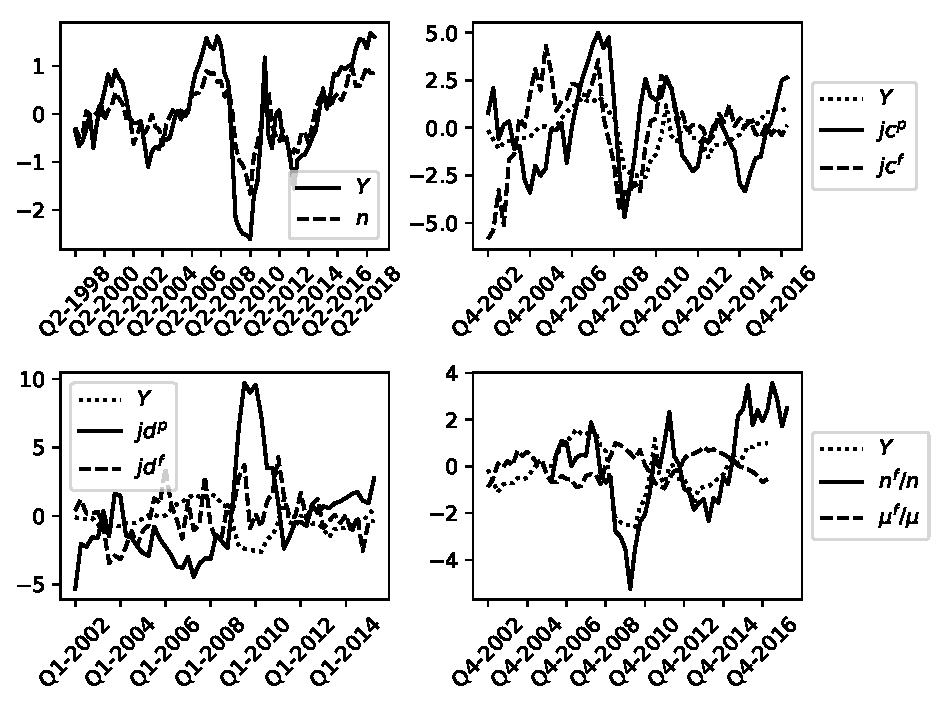
\includegraphics[scale=1.]{StylizedFacts.pdf}
\caption{Fluctuations in labor market values.}
\label{fluctuations}
\end{figure}

In this paragraph, we assess the ability of the model with respect to the reproduction of labor market moments. The absence of proper series for the computation of the latter in the Euro area represents a significant obstacle. As a result, I use French data series from \textit{Acoss - Urssaf} and \textit{Insee} as a proxy to account for the main features of the labor market.

The series are logged and filtered along the lines of Hamilton (2017) \cite{hamilton2017you}. Importantly, I do not use the so-called Hodrick-Prescott filter, whether it be one-sided or two-sided. Indeed, Hamilton (2017) explains the purely artifical statistical properties of series filtered through the Hodrick-Prescott method. The use of the Hodrick-Prescott filter imposes strong statistical properties on series because of its inner structure, regardless the process behind the actual data. Stunningly, when considering random walks, the output of the Hodrick-Prescott filter presents persistence. This behavior of the Hodrick-Prescott filter is all the more worrying since macroeconomic time series often boil down to martingales, whose increments remain unpredictable by definition. In standard macroeconomic samples of data, a band pass filter only captures the frequencies belonging to cycles with periodicity between 5 and 40 quarters. Considering growth rates exaggerates the high frequency margin in the data. Overall, a filtering method remains an arbitrary choice with many pitfalls\footnote{See Gorodnichenko and Ng (2010) \cite{GORODNICHENKO2010325}, Ferroni (2011), Lafourcade and De Wind (2012) \cite{lafourcade2012taking}, Canova (2014) and Hamilton (2017) for thorough developments of this idea}.

% Table generated by Excel2LaTeX from sheet 'Sheet1'
\begin{table}[t]
  \centering
  \caption{Actual and simulated correlations with output of labor market variables}
	\begin{tabular}{cccccc}
	\toprule
    \toprule
          & \multicolumn{2}{c}{Data} &       & \multicolumn{2}{c}{Model} \\
    	\cmidrule{2-3} \cmidrule{5-6}
          & Std. Dev. & $Cor(Y,.)$ &       & Std. Dev. & $Cor(Y,.)$ \\
    \midrule
    $Y$   & 0.51  & 1.00  &       & 0.36  & 1.00 \\
    $n$   & 0.32  & 0.93  &       & 0.41  & 0.86 \\
    $jc^p$ & 2.98  & 0.65  &       & 4.41  & 0.42 \\
    $jc^f$ & 2.07  & 0.43  &       & 2.36  & 0.48 \\
    $\mu^f / \mu$ & 0.56  & -0.46 &       & 0.85  & -0.26 \\
    $n^f / n$ & 0.83  & 0.09  &       & 0.89  & 0.39 \\
    $jd^p$ & 3.15  & -0.59 &       & 6.71  & -0.62 \\
    $jd^f$ & 1.32  & 0.38  &       & 1.00  & 0.06 \\
    $v$   & 6.50  & 0.87  &       & 3.47  & 0.51 \\
    \bottomrule
    \end{tabular}%
  \label{corr}%
  \begin{flushleft}
  \footnotesize{For each of the 10,000 particles from the SMC algorithm, the correlations are computed over 400-period chains of shocks after a 100-period burn-in time. A weighted average of these moments is then derived using the particle-specific weights generated by the SMC procedure.}
  \end{flushleft}
\end{table}%

Figure \ref{fluctuations} displays the fluctuations in output $Y$, employment $n$, job creation through permanent contracts $jc^p$ and temporary contracts $jc^f$, endogenous permanent job destruction $jd^p$ and temporary job destruction $jd^f$, the share of temporary contracts in the labor force $n^f / n$ and in job creation $\mu^f / \mu$. The Great Depression jumps out in these graphs. Employment is less volatile than output and is strongly pro-cyclical. Job creation through temporary and permanent contracts are equally volatile and pro-cyclical, and are more volatile than output. Job destruction series are strongly counter-cyclical and more volatile than output. Endogenous permanent job destruction varies more than temporary job destruction, which fluctuates more than output. These behaviors are well documented in the literature. 

The genuine novelty of this paper rests on the role of temporary contracts in front of fluctuations. The shares of temporary contracts in the labor force is counter-cyclical, while the shares of temporary contracts in job creation is pro-cyclical. The former is more volatile than output, whereas the latter displays less variability. During recessions, the share of temporary employment in total employment shrinks. This result is consistent with the buffer effect of temporary employment Saint-Paul (1996) described. Fixed-term contracts serve as an adjustment variable to avoid costly permanent workers' lay-offs. Interestingly, temporary employment represent a higher share of job creation in the doldrums. During downturns, the magnified probability of separation entails an increase in the expected loss through the firing costs when a permanent worker is hired, which explains the substitution towards temporary contract on behalf of permanent ones at the hiring stage.

Table \ref{corr} displays the correlation of these variables with output according to the data and the model. The model fits remarkably well the cyclical co-movements of the French dual labor market. The model underestimates the magnitude of the co-movements between output and the share of temporary contracts in job creation. The particularly strong share of temporary contracts in French job creation may explain the poorer fit of the model, which is rather calibrated and estimated to match the more tempered situation of the Euro Area as a whole. The standard deviations are properly matched, with the exception of permanent job destruction and vacancies, whose standard deviations are respectively overestimated and underestimated. These results are all the more encouraging that time series specific to dualism on the Euro area labor market were not used in the estimation process.

%Another possible explanation to the understatement of the model is the improper joint assumptions of constant standard deviations of shocks with the order-one log-linearization implemented here. Sensier and Van Dyck (2004), among others, demonstrated that crises were episodes with a high volatility. My data sample for the computation of moments precisely includes the 2008's crisis, whereas the model does not embed time-varying volatilities for shocks. Therefore, some of the volatility in the data cannot be accounted for in the reaction of temporary employment. The effect of macroeconomic volatility on a dual labor market is left for future research. 

%Another pitfall of the model consists in the improper fit of the standard deviations of the different series. The high standard deviation of the government spending shock is responsible for this failure. As a matter of fact, the government spending shock embodies all demand shocks that are not explicitly modelled here. Beyond government spending shocks, this may include shocks on investment, on exports or on prices of imported products for example. This problem mitigates when investment, capital, risk-aversion and habit formation are introduced in the same manner as Gertler et al. (2008) \cite{gertler2008estimated}. I preferred to display a simple model to insist on the economic phenomena specific to dual labour markets, which are relatively new in the DSGE literature. 

\subsection{Impulse Response Functions}

The computation of impulse response functions highlights several interesting features of the model. First of all, a substitution effect between temporary and permanent contracts emerges, with long-run consequences on employment whether it be temporary or permanent and a strong influence on impact. Secondly, a general-equilibrium effect appears. Indeed, shocks imply changes in the size of the job seekers' pool, which, in turn, has important implication for job creation flows. Finally, the common source of both effects being the evolution of $\left( z^p, z^f, z^*, \theta\right)$, the two effects interact through time depending on the persistence of the considered shock.

\begin{figure}[t]
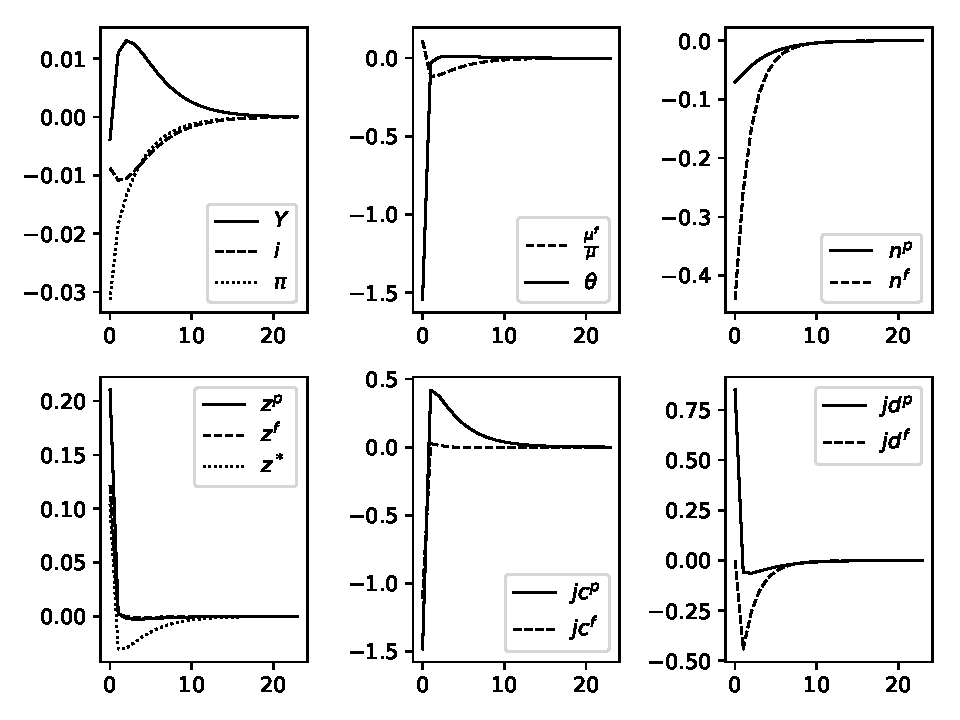
\includegraphics[scale=1]{IRF_A.pdf}
\caption{IRF of main variables to a one-standard-deviation productivity shock}
\label{IRF_A}
\end{figure}

\paragraph{Productivity shocks} Figure \ref{IRF_A} displays the reaction of main variables to a productivity shock. An increase in labor productivity cuts real marginal costs. Inflation decreases and the central bank reduces nominal interest rates to encourage consumption. The support to demand is insufficient to prevent a decrease in employment. Unemployment increases while vacancies reduce, delineating a downward-sloping Beveridge curve and a decrease in labor market tightness. These results are classic in DSGE models with nominal rigidities. The downward sloping Beveridge curve is a traditional feature of Mortensen Pissarides models.

The behavior of flows constitute an important feature of labor markets. The enhanced productivity fuels higher job destruction among permanent contracts ; $z^p$ increases. Firms are more reluctant to keep low-productivity permanent matches as their expected gain from searching a worker enlarges. Job creation, as for it, immediately decreases through both permanent and temporary contracts because of of the drop in labor demand. Interestingly, job creation ends up increasing a few quarters after the observed cut on impact. This comes from a general equilibrium effect. Just after the shock, aggregate job destruction increases and job creation shrinks, which inflates the job seekers' pool for the next periods. This mechanically increases the subsequent job creation flows. On impact, output decreases because of the shrink in employment, which overcomes the productivity gains. Thereafter, the recovery of job creation pushes it up. 

The movements in thresholds $z^f$ and $z^*$ are key. The enhanced productivity makes firms' hiring policy more stringent and worker-firm pairs are more exacting about the productivity of an accepted match when they meet ; $z^f$ enlarges. The forces at stake when it comes to the evolution of $z^*$ are more complex. On one hand, the agents seek to benefit from productivity gains in full, which bolsters the attractiveness of permanent workers. On the other hand, firms are more demanding in terms of productivity when hiring a new permanent worker. On impact, the latter effect prevails, but it is quickly overcome by the former. The choice between a temporary and a permanent contract at the hiring stage also reflects the compromise between the fear of future rigidity and the appetite for productivity gains. Overall, productivity gains are insufficient to encourage substitution in favor of permanent contracts ; the transitory nature of the shock encourages the resort to temporary contracts, and the share of temporary contracts in job creation increases\footnote{This behavior stems from the location $z^f$ and $z^*$ occupy on the support of the distribution of idiosyncratic shocks, which Figure \ref{pdf} shows. Movements in $z^f$ concern more formerly viable matches than similar movements in $z^*$, the slope of the probability density function of idiosyncratic shocks being higher in the neighborhood of $z^f$.}. Permanent employment unambiguously shrinks under the joint diminution in job creation and increase in job destruction. As for temporary contracts, job creation shrinks and job destruction occurs at a constant exogenous rate. Consequently, temporary employment decreases. 

\begin{figure}[t]
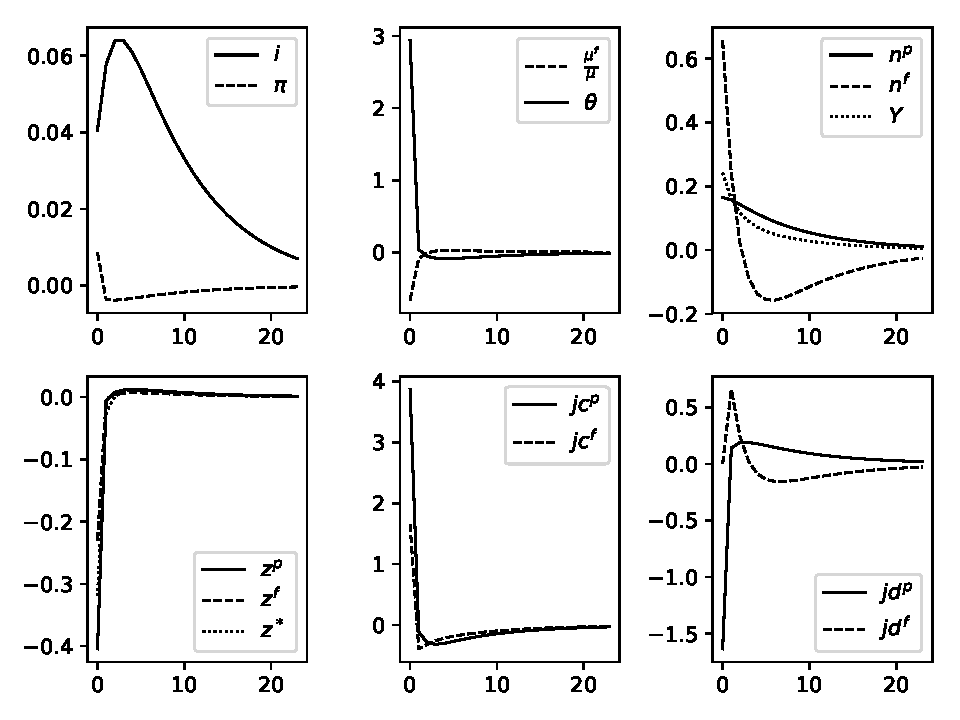
\includegraphics[scale=1]{IRF_g.pdf}
\caption{IRF of main variables to a one-standard-deviation shock in government spending shock}
\label{IRF_g}
\end{figure}

\paragraph{Government spending shocks} Figure \ref{IRF_g} shows the impulse response functions of main variables after a shock in government spending. As usual in the literature, a sudden increase in government spending enhances output. Real marginal costs increase and the central bank increases the nominal interest rate to prevent the spread of inflation. The labor market tightness increases as firms post more vacancies to cope with the magnified demand of consumption goods. As a result, on impact, job destruction decreases and job creation increases. Interestingly, firms cope with the surplus of demand through an enlarged share of permanent contracts in job creation. The shock is persistent enough for the future expected losses associated with firing costs to be overcome by lifelong productivity gains. The general-equilibrium effect described in the preceding sections weighs in anew. Indeed, the shrink in the job seekers' stock exerts a downward pressure on job creations, which decrease below their steady-state values. While the transitional path of permanent employment remains above its steady-state value, temporary employment goes below its equilibrium level. As a matter of fact, fixed-term employment experiments a higher turnover, and is therefore highly impacted by temporary fluctuations in its associated job creation\footnote{This is all the more true since destruction rates of temporary jobs are constant}.

\begin{figure}[t]
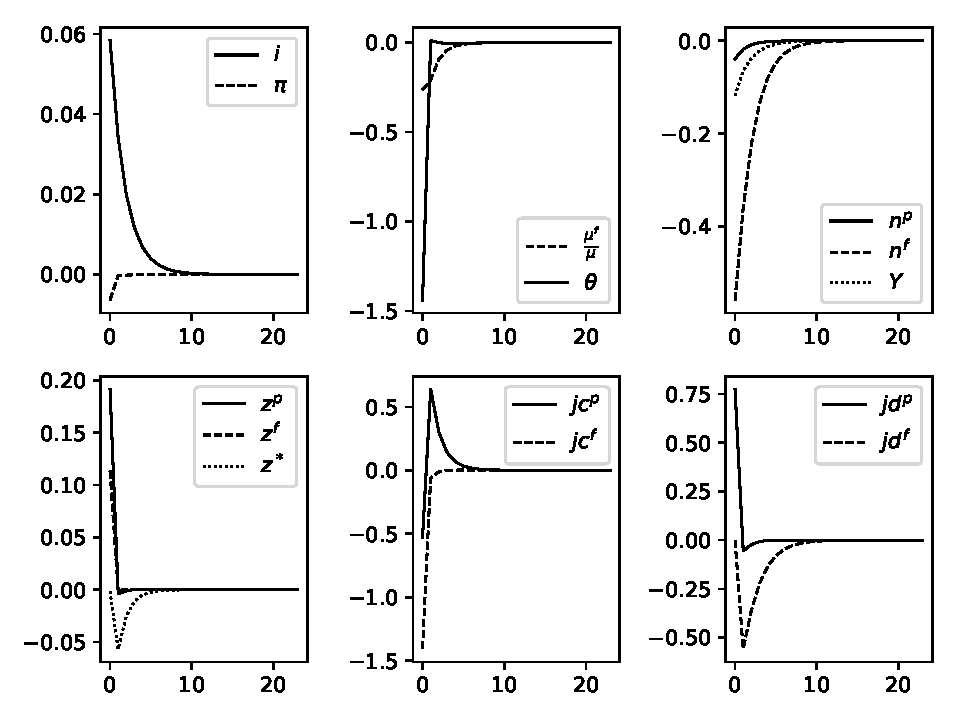
\includegraphics[scale=1]{IRF_m.pdf}
\caption{IRF of main variables to a one-standard-deviation in the monetary policy shock}
\label{IRF_m}
\end{figure}

\paragraph{Monetary policy shock} Figure \ref{IRF_m} shows the impulse response functions of main variables after a shock in the monetary policy. A monetary policy shock pushes up interest rates, which discourages consumption and subsequently depresses output. Real marginal costs and inflation decrease. The marginal gross revenue from labor decreases and intermediate firms are overall more demanding in productivity terms to compensate the loss in profits ; firms post fewer vacancies and $z^p$ as well as $z^f$ increase. Thus, on impact, the labor market tightness shrinks and permanent job destruction enlarges. In turn, the formerly permanent employees join the ranks of the job seekers', which enhances job creation. Moreover, firms tend to switch to permanent contracts on behalf of temporary ones at the hiring stage in order to temper the immediate loss in revenue due to prices ; $z^*$ decreases. These two effects combined explain the observed rebound in permanent job creation.

As a result, viewed from the labor market, the monetary policy shock represents the negative of the government spending shock. The economic schemes at stake are the same. There is however a nuance. The effects of the monetary policy shock on the interest rate vanish much faster and the oscillations between the substitution effect and the general-equilibrium effect develop in a rougher way. This observation is also relevant when one considers the cost-push shock. The IRF of the latter will not be described, as it involves the same economic phenomena as the other shocks.

\subsection{Reforms in employment protection legislation}

In this paragraph, I examine the macroeconomic effects of a reform on employment protection legislation, which is summed up in firing costs here. I consider both transitory and permanent shocks. Transitory shocks are interesting, as employment protection legislation has frequently been the target of many reforms in Europe. Fontaine and Malherbet (2016) \cite{fontaine2016cdd}, quoting a report from an observatory of the European Commission, mention the implementation of more than 220 policies related to employment protection legislation between 2005 and 2013. Permanent shocks, as for them, are relevant to study changes in volatilities of inflation, employment or output for example.

\begin{figure}[t]
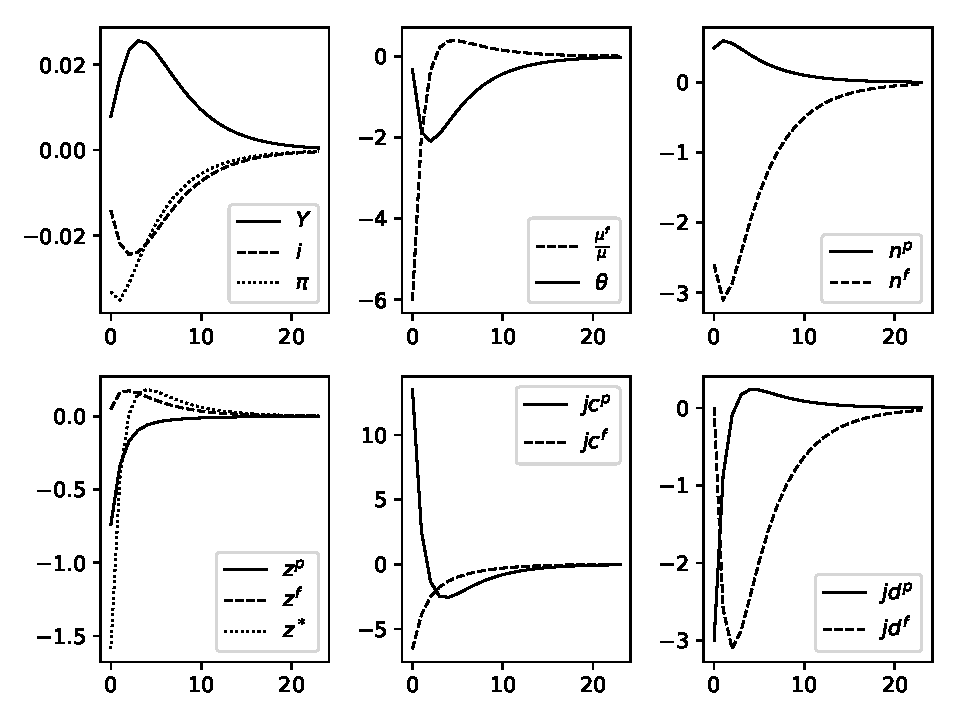
\includegraphics[scale=1]{IRF_F.pdf}
\caption{IRF of main variables after a one-per-cent shock in firing costs}
\label{IRF_F}
\end{figure}

Figure \ref{IRF_F} displays the reaction of main variables to a one-percent positive shock to firing costs. The process for the logged shock is supposed to be an AR(1) with auto-regressive coefficient 0.8, so that the shock vanishes at 99\% five years after the impact. An increase in firing costs discourages job destruction ; $z^p$ and $jd^p$ decrease. Two opposite effects weigh on the composition of job creation. On one hand, enlarged firing costs entail costlier endogenous separations, which encourages substitution towards temporary job creation. On the other hand, these endogenous separations are scarcer. As a result, firms are less demanding in terms of productivity when it comes to hiring a permanent worker, which favors substitution towards permanent employment. In the present case, the latter effect prevails ;  the share of temporary contracts in job creation diminishes. This is not surprising since, at steady state, costly separations only represent 30 \% of all separations. The rigidity effect would probably dominate if all separations entailed a red-tape cost. This phenomenon is particularly relevant to the policymaker.

Interestingly, the expected gain from posting a vacancy decreases because of the shrinking average productivity of hired permanent workers and labor market tightness decreases. The resulting increase in vacancy-filling rate joint with the loosened threshold for permanent hires overcome the depressed number of vacancies and permanent job creation expands. The reduced job destruction rate and the increase in job creation account for the increase in permanent employment. The substitution effect towards permanent contracts depresses temporary job creation and temporary employment, as temporary job destruction occurs at a constant rate. Overall, output increases. Inflation decreases with real marginal costs ; the decrease in the average productivity makes intermediate goods more expensive, but the higher vacancy-filling probability fueled by a lower labor market tightness overcomes this negative effect. The central bank cuts interest rates in response to the decrease in inflation. Interestingly, a temporary reform generates long-lasting effects on inflation.

\begin{figure}[t]
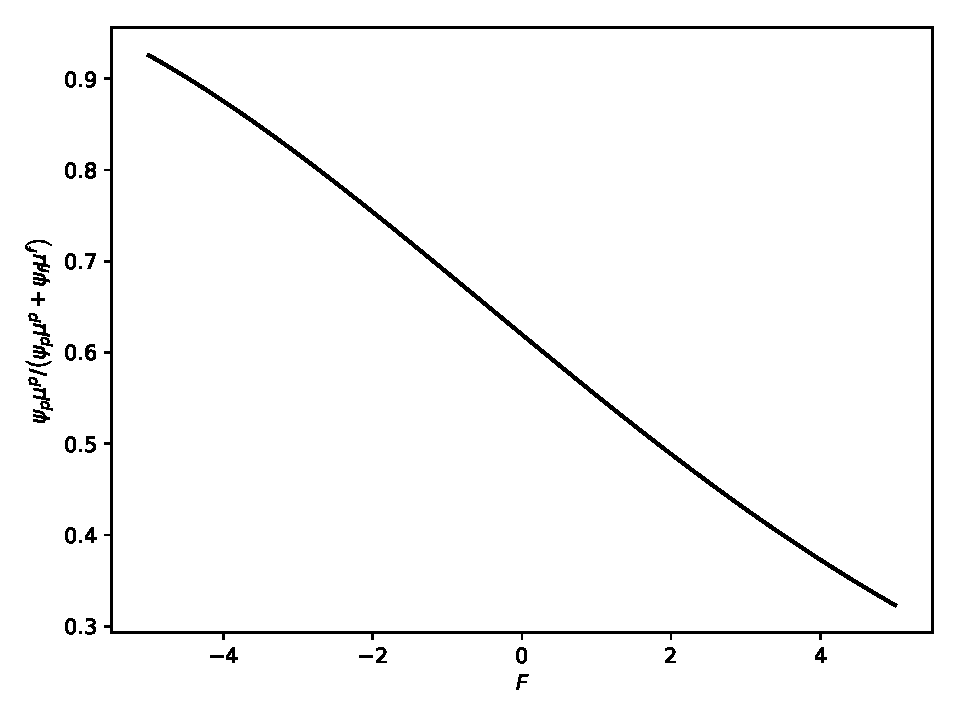
\includegraphics[scale=1]{NKPC.pdf}
\caption{The weight of permanent contracts in inflation dynamics in function of steady-state firing costs.}
\label{NKPC}
\footnotesize
\begin{flushleft}
The x-axis represents the percentage deviation of steady-state firing costs with respect to the baseline calibration, which is set at 0.
\end{flushleft}
\end{figure}


In order to understand the dynamics of inflation, I derive the New-Keynesian Phillips curve associated with the present model as is classic in the literature and find

\begin{align*}
\widehat{\pi_t} = \beta \mathbb{E}_t \widehat{\pi_{t+1}} + \kappa \left( \widehat{\mu_t} + \widehat{\phi_t} \right)
\end{align*}

where $\kappa = (1-\beta \psi) (1-\psi) / \psi$.

Meanwhile, I use the job creation condition to isolate $\phi_t$ and obtain

\begin{align*}
\phi_t = \frac{\gamma}{ (1-\eta) A_t \left[ \left( E_z \left[ z \middle| z \geq z_t^* \right] - z_t^c \right) q\left( \theta \right) \left( 1 - G\left( z_t^* \right)\right) + \rho \left( E_z \left[ z \middle| z_t^f \leq z \leq z_t^* \right] - z_t^f \right) q\left( \theta \right) \left( G\left( z_t^* \right) - G\left( z_t^f \right)\right) \right] }
\end{align*}  

The left-hand-side term in the bracketted part of the denominator is the expected surplus of production from a hire through permanent contract $\psi_t^p$ weighted with its probability of occurence $\mu_t^p$. This so-called surplus of production is the production of the match beyond the one corresponding to the zero-profit point. In an analogous manner, the right-hand-side term is the expected surplus of production from a hire through a temporary contract $\psi_t^f$ weighted by its probability of occurence $\mu_t^f$. Overall, the real marginal cost evolves negatively with the ability of the labor market to generate in expectations such production surpluses. This reminds the simple rule of a decreasing cost with respect to the abundance of a given good. Log-linearizing this condition and assuming that there are neither cost-push shocks nor productivity shocks, the New-Keynesian Phillips curve becomes

\begin{align*}
\widehat{\pi_t} = \beta \mathbb{E}_t \widehat{\pi_{t+1}} - \kappa \frac{\mu^p \psi^p}{\mu^p \psi^p + \mu^f \psi^f} \left( \widehat{\mu_t^p} + \widehat{\psi_t^p} \right) - \kappa \frac{\mu^f \psi^f}{\mu^p \psi^p + \mu^f \psi^f} \left( \widehat{\mu_t^f} + \widehat{\psi_t^f} \right)
\end{align*}

Retailers benefit from their market power and extract a rent from the production that exceeds intermediate firms' profitability thresholds. Interestingly, the discounted innovation in inflation is a weighted average, with the steady-state share of the newly hired workers' production for each contract as weights. The magnitude of these weights is difficult to assess, to the extent that they reflect a trade-off between a high hiring probability and a low average productivity, and conversely. The determinants of inflation dynamics are directly related to the evolution of the contractual composition of hires and their productivity. Figure \ref{NKPC} shows the importance of fluctuations on the permanent side of the labor market with different values of $F$, 0 being the baseline calibration. When $F$ increases, the weight of permanent contracts in the shaping of inflation dynamics decreases. As permanent job destruction becomes scarcer, the agents are less exacting in the productivity of hired permanent workers, which overcomes the enhanced permanent job creation ; the permanent side of the labor market loses importance when considering inflation dynamics. Importantly, these results highly depend on the distribution of idiosyncratic shocks. Nevertheless, as we changed $\sigma_z$ to 0.1 or 0.15, there were no notable difference in the results\footnote{An interval of values for the standard deviation of distribution of idiosyncratic productivity shocks $\sigma_z$ over which steady-state quantities are plausible is $( 0.1 , 0.22 )$}. Another important factor that influences inflation dynamics is the adjustment speed of employments, which is small in a labor market where flows are constrained by employment protection legislation. Consequently, reforms in employment protection legislation generate significant and persistent fluctuations in inflation. The size of the subsequent perturbations is small, though. A 10-per-cent cut in firing costs typically entails a 30-basis-point decrease in inflation on impact.

\section{Conclusion}

In this paper, I show the importance of the contractual composition with respect to labor market flows when it comes to understand fluctuations on a dual labor market. The estimated model replicates well the main moments of a typical European dual labor market. Our approach highlights the importance of a contractual substitution effect at the hiring stage and the general-equilibrium effect it fuels by impacting the job seekers' pool. Inflation dynamics reflect the firms' hiring choices in contractual terms. As a result, employment protection legislation reforms directly impact inflation dynamics.

A few points merit further discussion, though. A genuine problem in the current analysis is the implicit assumption that the labor market \emph{is} at the steady state. According to the data, temporary employment in the Euro area seems to have stabilized since the beginning of the 2000s, but the exponential rise of temporary employment between the 80s and 2000 may cast doubt on its future behavior. The absence of endogenous quitting decisions is also a limitation that needs to be highlighted, especially in the Euro Area where voluntary job-to-job transition represent a substantial share of permanent job separations and probably present a sharp pro-cyclical behavior. The exogenous character of the productivity distribution and its independence of other shocks also constitutes a problem, because this makes the model sensitive to the Lucas critique. Indeed, an employment protection legislation reform probably modifies firms' productivity distribution. With these critiques in mind, my findings should be considered as an humble incentive to consider the contractual composition of labor market flows in an endogenous manner, as substitution effects between contracts at the hiring step play an essential role in labor market dynamics.

%Shocks are i.i.d for the sake of simplicity. 

\bibliographystyle{acm}
\bibliography{sources}


\end{document}